\documentclass{article}

\PassOptionsToPackage{square,numbers}{natbib}

\usepackage[final]{neurips_2024}


% to compile a preprint version, e.g., for submission to arXiv, add add the
% [preprint] option:
%     \usepackage[preprint]{neurips_2024}


% to compile a camera-ready version, add the [final] option, e.g.:
%     \usepackage[final]{neurips_2024}


% to avoid loading the natbib package, add option nonatbib:
%    \usepackage[nonatbib]{neurips_2024}


\usepackage[utf8]{inputenc} % allow utf-8 input
\usepackage[T1]{fontenc}    % use 8-bit T1 fonts
\usepackage{hyperref}       % hyperlinks
\usepackage{url}            % simple URL typesetting
\usepackage{booktabs}       % professional-quality tables
\usepackage{amsfonts}       % blackboard math symbols
\usepackage{nicefrac}       % compact symbols for 1/2, etc.
\usepackage{microtype}      % microtypography
\usepackage{xcolor}         % colors

\usepackage{csquotes}
\usepackage{graphicx}
\usepackage{amsmath}
\usepackage{multirow}


\title{Formatting Instructions For NeurIPS 2024}


\author{
  Maël Dieudonné\\
  ENSAE\\
  \texttt{mael.dieudonne@ensae.fr} \\
}


\begin{document}

\maketitle

\begin{abstract}
  The abstract paragraph should be indented \nicefrac{1}{2}~inch (3~picas) on
  both the left- and right-hand margins. Use 10~point type, with a vertical
  spacing (leading) of 11~points. The word \textbf{Abstract} must be centered,
  bold, and in point size 12. Two line spaces precede the abstract. The abstract
  must be limited to one paragraph.
\end{abstract}


\section{Introduction}

Sentiment analysis seeks to understand the subjectivity expressed in written documents. Opinion and views are often used interchangeably with sentiment in the literature, in contrast to factual statements \citep{munezero_are_2014}.

Sentiment analysis has become an active research area with the advent of Web 2.0, offering people numerous opportunities to express themselves in a publicly traceable manner \citep{stine_sentiment_2019}. Various stakeholders have a vested interest in their opinions:
\begin{itemize}
\item Marketing departments, seeking to understand brand perception and consumer opinions about products, both in absolute terms and relative to competitors.
\item Customer service teams, identifying key factors contributing to customer satisfaction or dissatisfaction.
\item Traders and financial analysts, using public sentiment as an early indicator of economic trends and the financial health of companies.
\item Political actors, monitoring public perception of policies and personal image.
\item Public health officials, assessing attitudes toward medical interventions such as vaccines.
\item Etc.
\end{itemize}

The primary goal of sentiment analysis is to gain direct access to people's opinions without relying on intermediaries such as journalists or resellers, at the massive scale typical of the Internet \citep{ravi_survey_2015,hemmatian_survey_2019}.

Sentiment analysis can be performed at three distinct levels. At the document level, the goal is to determine the overall sentiment of an entire document, which can be very short (e.g., product reviews). Analysis conducted at the sentence level account for potentially conflicting sentiments within the same documents. First, it distinguishes between objective (fact-based) and subjective (opinion-based) sentences. For example, a movie review may contain both plot summaries (objective) and judgments on acting performance (subjective). Then, subjective sentences are classified based on their sentiment. At the feature or aspect level, the aim is to link sentiments with their object, and sometimes the person expressing them (who feels what about the plot, for instance).

The most common output of sentiment analysis is a binary or ternary classification of the emotional tone, also known as polarity or valence: positive, negative or neutral. This classification applies to entire documents, individual subjective sentences, or specific features, depending on the level of analysis. Sentiment classification beyond polarity, aiming at identifying specific emotions like fear, anger, or happiness, is less common. This approach may have fewer applications outside of literary analysis.

Sentiment analysis faces several challenges \citep{kumar_comprehensive_2023}:
\begin{itemize}
    \item Domain dependance, when words carry different meanings in different contexts (e.g., tears may indicate laughter or sadness).
    \item Polarity shift, when words or punctuation marks change the valence of a sentiment (e.g., not, but, only).
    \item Sarcasm, when the expressed sentiments oppose the actual sentiments.
    \item Order dependance, when the valence of a word changes with its position in the sentence (e.g., with comparisons).
    \item Unconventional expressions like idioms, slang, emojis, or multiple punctuations marks.
Implicit sentiment, when sentiments are expressed without explicit sentiment words (e.g., “I know real Indian food and this wasn’t it”).
\end{itemize}


\section{State of the art}

Three main approaches have been applied to sentiment analysis \citep{hartmann_more_2023}:
\begin{enumerate}
    \item Lexicon-based
    \item Classifiers
    \item Transformers
\end{enumerate}

\subsection{Lexicon-based}

This approach relies on a dictionary assigning positive or negative labels to words, to classify documents based on the most frequent label. A well-known example is VADER, which was developed to analyze the sentiments of reviews published on social media \citep{hutto_vader_2014}. It relies on sentiment lexicon of 7520 words including slang, emoticons, and acronyms, where each word is associated with a score on a valence scale (e.g., -2.2 for ':(', 0.9 for 'okay' or 3.1 for 'good'). This lexicon was obtained by submitting a list of 9,000 words to human raters recruited on the Amazon Mechanical Turk. Each word was rated by 10 different persons on a 9-point Likert scale, and kept in the lexicon if its average rating was non-null. VADER also applies rules that adjust sentiment scores based on punctuation, capitalization, and specific words (e.g., 'but' shifts sentiment, while '!!' amplifies intensity). Finally, VADER calculates the proportion of text conveying positive, negative, or neutral sentiment.

This approach has several limits. Lexicons are complex to build, as they require a lot of human input, so they tend to remain small and not updated very often. They also lack flexibility, being unable to handle words they do not include. This can be especially problematic when processing content drawn from the Internet, which may include words written incorrectly or with evolving meaning. Since the analysis occurs at the word level, it lacks contextual understanding. As a result, the performance of lexicon-based sentiment analysis is rather low.

\subsection{Classifiers}

A second approach consists of using standard machine learning algorithms. Almost any classification algorithm can be applied; the challenge lies in preprocessing the text to make it suitable for the classifier, typically through a bag-of-words representation. This method produces a high-dimensional but sparse feature space, making regularization techniques particularly useful. These techniques reduce the vocabulary—similar to a lexicon—but do so based on a word’s effectiveness in sentiment prediction rather than a predefined list. An example is available here with support vector machines, random forest and neural networks \citep{wang_is_2024}.

The use of classifiers can be seen as a generalization of lexicon-based approaches. Unlike lexicon-based methods, classifiers do not require a predefined dictionary specifying which words to consider and how to interpret them. Instead, models autonomously select the words they rely on for classification, along with their associated sentiment (i.e., emotional tone). They enable more complex mappings between the input (i.e., document) and the output (i.e., predicted sentiment) beyond simple relative word frequencies. Classifiers can also incorporate external features, such as a reviewer’s personal characteristics, to refine predictions.

However, classifiers have limitations. They require labeled datasets to train the models, though these datasets are generally easier to construct than sentiment dictionaries. Despite their advantages, classifiers may still struggle with understanding connotations and context, as they analyze words in isolation. While they perform well on short documents, they often have difficulty handling longer texts that express conflicting viewpoints.

\subsection{Transformers}

The third approach uses transformer models, which apply attention mechanisms to word embeddings—low-dimensional, dense representations of text. There are two main types of models sharing the same basic architecture:
\begin{itemize}
    \item Encoder/decoder (a.k.a. unidirectional or autoregressive transformers): These models consider only past and present tokens, with the aim of predicting future tokens (which are removed from through causal masking). They are easily trained by comparing predicted and actual tokens. The reference architecture for this type is GPT \citep{radford_improving_2018,radford_language_2019}.
    \item Encoder-only (a.k.a. bidirectional transformers): These models consider all tokens in the context window, with the aim of understanding text. They are trained by masking a fraction of input tokens (usually 15\%) before feeding them to the model, then predicting the masked tokens. Additional training strategies include predicting the order of two sequences in the training corpus or generating permutations of tokens within sentences. Lacking decoders, these models output embeddings instead of tokens. These embeddings can be analyzed directly, e.g., through cosine similarity to identify semantically similar tokens, which is essentially the principle of zero-shot classification. Alternatively, a custom output head can be added and fine-tuned for a specific task. The reference architecture of encoders is BERT \citep{devlin_bert_2019}.
\end{itemize}

Large Language Models offer powerful tools for sentiment analysis, with a unique ability to capture context and disentangle sentiment from other features. They excel in complex tasks, particularly aspect-based sentiment analysis. However, they have several limitations. They are resource-intensive, especially during pre-training. As a result, the most common approach is to use pre-trained encoders models, either directly or for fine-tuning. A less frequent approach is to run GPT models locally or access them via APIs. One challenge with transformers is their opacity; what makes them so effective remains difficult to assess. Lastly, they may not outperform traditional classifiers on short documents \citep{ghatora_sentiment_2024}.


\section{Data}

Movie reviews have become a popular benchmark for sentiment analysis due to their availability and size: they tend to be longer and more accessible online compared to typical product reviews or social media posts. The current dataset was constructed and publicized by Maas et al. \citep{maas_learning_2011}. It contains 50,000 reviews from the IMDb website, along with the corresponding rating proposed by theirs authors on a 1-10 scale. Reviews are labeled as negative when associated with ratings \( \leq 4 \), as positive when associated with ratings \( \geq 4 \). Neutral ratings (5 and 6) were eliminated to focus on polarized reviews. To eliminate bias, no more than 30 reviews per movie were included, and an even number of positive and negative reviews were included, so that randomly guessing yields 50\% accuracy. To minimize bias, no more than 30 reviews per movie were included, and an equal number of positive and negative reviews were selected, ensuring that random guessing would yield 50\% accuracy. The dataset is split into training and test sets of equal size (25,000 reviews each) 
\footnote{The dataset also includes an additional 50,000 unlabeled reviews without ratings. These can be used for unsupervised learning but not to measure performance.}
.

The task, therefore, is to perform binary classification between positive and negative sentiments at the document level.

\subsection{Benchmarks}

Performances are assessed regarding accuracy, which is the most relevant metrics for a binary classification problem where each class is of equal importance and the dataset is balanced. This is different from, e.g., diagnosing a serious but rare disease, where false positives are preferable to false negatives, and recall would be the performance metric of choice.

Several models were benchmarked on the IMDb dataset, reaching the following error rates on the test sample \citep{stine_sentiment_2019}:
\begin{itemize}
    \item 26.4\% for a lexicon-based model,
	\item 12.3\% for a Lasso logistic regression,
	\item 5.91\% for an adversarial neural network.
\end{itemize}

The current best model (according to the \href{https://paperswithcode.com/sota/sentiment-analysis-on-imdb}{Papers with Code leaderboard}) is a fine-tuned BERT model named LlamBERT (Csanády et al., 2024) with an error rate of 3.32\%. It is followed closely by an auto-regressive transformer named XLNet (Yang et al., 2019) with an error rate of 3.79\%.

Transformers are significantly outperforming lexicon-based models and traditional classification algorithms. This is not surprising, as they leverage much more information, being trained on corpora orders of magnitude larger than the IMDb dataset. However, they seem to have reached a plateau, with only marginal improvements over the last 6 years. However, they appear to have reached a plateau, with only marginal improvements over the past six years. Additionally, they are difficult to replicate due to heavy hardware requirements. It seems clearly out of my reach to improve upon or even replicate these models.

\section{Experiment}

\subsection{Hypotheses}

Instead, I have set out to investigate the possibility that performance is plateauing due to limitations of the dataset, with two hypotheses in mind.

(1) The rating is not a good proxy for the overall sentiment of reviews. See a few example of reviews labelled as positive, while their tone is quite ambiguous:
\begin{displayquote}
Definitely a movie that could've been seen on DVD. (rating 7)

Moviegoers wanting an inside look at what it's like to embark on a daring rescue mission in the middle of the ocean might want to give The Guardian a chance. I saw it for free, but had I paid I would've felt I had gotten my money's worth. (rating 8)

In the end, "The Dresser" will bore many people silly, but it will truly be a delight to those who love British cinema. (rating 8)

The theme is controversial and the depiction of the hypocritical and sexually starved india is excellent.Nothing more to this film.There is a lack of good dialogues(why was the movie in english??). There was lack of continuity and lack of passion/emotion in the acting. (rating8)
\end{displayquote}
The working hypothesis here is that the error rate is higher for models closer to neutral, especially with a rating of 7.

(2) Document level is not appropriate, because many reviews express conflicting opinions regarding different aspects of the films.
\begin{displayquote}
Some things and some actions are very true, but some other stuff is just way off the mark. (…) Delhi is complicated. India is complicated. The director tries to simplify both. And fails pretty miserably at that. (…) But the chemistry between the leads is palpable. (rating 8)

The plot is rather thin, yet it does have a moral. It's about the perils of quick fame and fast money, and how any happiness with only these factors will ultimately be doomed. This will cheer you up, lift you up to your feet and make you laugh. (…) Another major problem is that too many songs are just not that great. (…) The grandmother sub-plot borders on being ridiculous. (rating 8)
\end{displayquote}
The working hypothesis here is the lengthier the reviews, the more likely they are to express contrasted opinions, and the harder they become to classify.

\subsection{Models}

My goal was to compare several models to assess their behavior in relation to ratings and review lengths, while striving to get as close as possible to the state-of-the-art (SOTA) performance. I chose RoBERTa Large as my base model \citep{liu_roberta_2019}, since the SOTA model is built upon it and it also performs really well on its own (outperforming XLNet, which serves as the basis for the second SOTA model) 
\footnote{It could have been interesting to use ModernBERT \citep{warner_smarter_2024} instead, which is more recent, but I discovered its existence too late.}
.

RoBERTa's architecture is largely similar to the original BERT model, with only minor tweaks to some hyperparameters. It has a vocabulary size of 50,265, a hidden size of 768 for RoBERTa base and 1024 for RoBERTa large, 12 attention heads with 12 layers each and an intermediate size of 3072. The context length is 512 tokens. The sole difference between BERT and RoBERTa architectures regards tokenization. RoBERTa uses Byte-Pair Encoding, which operates at the subword level with an agglomerative approach, merging the most frequent pairs iteratively until the desired vocabulary size is reached. Additionally, RoBERTa omits \texttt{token\_type\_ids}, which are used in BERT to distinguish between prompts and answers.

Where BERT and RoBERTa truly differ is in their training procedures. RoBERTa eliminates the next sentence prediction objective and employs dynamic masking, meaning that input tokens are masked differently every 4 epochs rather than being fixed during preprocessing. Additionally, RoBERTa's training algorithm uses larger mini-batches and significantly fewer training steps (30,000 compared to 1 million for BERT). Its training corpus is also substantially larger, at approximately 160 GB. While I could not confirm whether it includes the IMDb dataset, it does use OpenWebText, which is built from content extracted from URLs shared on Reddit with at least 3 upvotes.

I use zero-shot classification with the base RoBERTa model through a simple HuggingFace pipeline as a baseline for performance, comparing it with the following models.

\subsubsection{Fine-tuned RoBERTa on the IMDb dataset}

I used a custom classification head with… 
\begin{itemize}
    \item A dense layer mapping RoBERTa output to a hidden space of similar size (making for \( 1024*1024+1024=1,049,600 \) trainable parameters)
	\item A drop-out layer with a rate of 0.1 to prevent overfitting
	\item An activation layer with GELU (same as RoBERTa) to introduce non-linearities
	\item A normalization layer (making for \( 1024*2=2,048 \) trainable parameters)
	\item A dense layer reducing the hidden space dimension by a factor 2 (making for \(1024*512+512=524,800\) trainable parameters)
	\item Another dropout layer with the same rate
	\item A final dense layer projecting the hidden space in 2 dimension, corresponding to binary outcomes (making for \(512*2+2=1,026\) trainable parameters)
\end{itemize}
This classification head has 1,577,474 trainable parameters in total, compared with 354,315,266 parameters in RoBERTa-large. It is applied to the \texttt{[CLS]} token, which marks the beginning of input sequences and serves as an embedding for their entirety
\footnote{I have tried applying it to the whole input sequence, pooling tokens through their mean or max, on a subset of reviews: the performance were worse.}
.

Parameters from the base model were frozen to preserve the knowledge acquired during pretraining and avoid excessive computation times. The fine-tuning was conducted with the following settings:
\begin{itemize}
    \item 12 epochs, with performance evaluation on the entire test set after each epoch to detect overfitting as soon as possible.
	\item An \texttt{AdamW} optimizer with a learning rate of 1e-4, \texttt{weight\_decay} of 0.03, and \texttt{epsilon} set to 1e-6.
    \item A cosine learning rate scheduler with 10\% warmup steps.
\end{itemize}

\subsubsection{SOTA fine-tuned RoBERTa for sentiment analysis}

To assess the effectiveness of my fine-tuning, I compared it not only to the baseline performance but also to the current SOTA fine-tuned RoBERTa for sentiment analysis, provided it was not trained on the IMDb test set. This model is SiEBERT \citep{hartmann_more_2023}. Its architecture is not specified, as the authors do not describe it and have not released their code. It is unclear whether SiEBERT uses a custom classification head or the default untrained head provided by RoBERTa, which consists of two dense layers (the first mapping to a hidden space of the same size as the RoBERTa output, the second to a binary space). The training corpus is also unspecified; the authors only mention using all publicly available two-class sentiment datasets they could identify, excluding their training subset.

SiEBERT is available in a HuggingFace pipeline, which I used.

\subsubsection{GPT 3.5 turbo}

I decided to add a comparison with ChatGPT, which has shown promising results for sentiment analysis but has never been applied to the IMDb dataset \citep{wang_is_2024}. I drafted a first prompt based on the principle of few-shot prompting, which consists in including a few examples before the document to classify. This has been observed to improve the performance of sentiment analysis significantly—an effect known as in-context learning \citep{brown_language_2020}. I then submitted this prompt to ChatGPT, asking for improvements, and received the suggestion of adding detailed instructions. Prompts were constructed as follows for each review of the test dataset:

\begin{displayquote}
Here is an example of a positive movie review, associated with a rating of 10:

*[ \textit{<random review with a positive sentiment from the training set>} ]*

Here is an example of a negative movie review, associated with a rating of 2:

*[ \textit{<random review with a negative sentiment from the training set>} ]*

Now, consider the following review. Based on its content, is the sentiment of the review positive or negative? Answer with a single word.

*[ \textit{<review to classify from the test set>} ]*

Instructions:

- **Positive** reviews typically highlight enjoyment, satisfaction, or praise for aspects of the film (e.g., acting, storyline, direction).

- **Negative** reviews tend to criticize the film for its shortcomings or failures (e.g., poor pacing, bad acting, or unsatisfying plot).

- Focus on the general tone of the review as a whole, not isolated statements or minor contradictions.
\end{displayquote}

I queried ChatGPT through the OpenAI API, which was terribly slow, averaging 7 seconds per call. I chose GPT 3.5 Turbo as the best compromise between cost and performance. At \$0.5 per million input tokens and \$1.5 per million output tokens, with 25,582,485 input tokens from building the prompt and 25,000 expected output tokens, the estimated cost was \$12.83.

An inherent challenge with this approach is data leakage. There is a high likelihood that the IMDb test set was included in GPT-3.5 Turbo's training corpus, which could lead to overestimated performance, as it may not be working with truly unseen data. The solution would have been to build a new dataset by scrapping reviews published after the cutoff date of GPT 3.5 Turbo, which is September 2021, but this would have added significant complexity to the project. Instead, I assumed that the IMDb dataset is small enough to be diluted in the larger training corpus of GPT-3.5 Turbo, making significant memorization unlikely.

\subsection{Data preprocessing}

Text was cleaned consistently across all models to ensure comparability of their results:
\begin{itemize}
    \item Removing HTML markups, primarily line breaks (replacing \texttt{<br>} with \texttt{\textbackslash n} to preserve the paragraph structure).
	\item Removing a few emojis that are not linked to sentiment (® and ©).
    \item Replacing hexadecimal characters by their ASCII equivalent.
\end{itemize}

\section{Results}

\subsection{Data}

Two characteristics of the dataset are not mentioned in the documentation but crucial nonetheless.
\begin{enumerate}
    \item A cursory examination suggests that movies are different in each dataset, even if they share the same id. This is excellent for preventing data leakage between train and test samples.
	\item All reviews goes in pair, with each movie having exactly one positive and one negative review. This forbids the models from learning non-sentiment-related features (e.g., related to the plot of a movie having overwhelmingly positive reviews in the dataset).
\end{enumerate}

The reviews are highly polarized, with nearly half of the dataset consisting of ratings of 1 or 10. The distribution of ratings is almost identical in both the train and test datasets. Most reviews are relatively short, but there is a long tail in the distribution of review lengths. Some reviews are exceedingly long, with a maximum of 2,459 words (for an average of 231 words in the train dataset, 223 in the test dataset). Review length and ratings are almost uncorrelated, with a Pearson correlation coefficient of 0.0148. This indicates that my two hypotheses can be tested independently.

\subsection{Candidate Labels for Zero-Shot classification with RoBERTa}

The initial run with 'positive' and 'negative' as candidate labels yielded relatively low accuracy. To improve performance, I experimented with more informative candidate labels. The best results were achieved using 'good movie' and 'bad movie' as labels, which resulted in an improvement of nearly 7 percentage points in accuracy compared to the 'positive' and 'negative' labels.

\begin{table}
  \caption{Performance of various candidate labels for zero-shot classification with RoBERTa}
  \label{tab:labels_zero_shot}
  \centering
  \begin{tabular}{lc}
    \toprule
    Candidate Labels & Accuracy \\
    \midrule
    positive sentiment / negative sentiment & 0.83056 \\
    positive / negative & 0.85908 \\
    favorable opinion / unfavorable opinion & 0.87596 \\
    positive review / negative review & 0.89136 \\
    excellent / terrible & 0.91140 \\
    good movie / bad movie & 0.91708 \\
    \bottomrule
  \end{tabular}
\end{table}

\subsection{Truncation}

RoBERTa models have a context length of 512 tokens, but many reviews are longer than that. The easiest solution is to truncate them, even though that means loosing part of the information on their overall sentiment. This truncation can be made from the right, keeping the end beginning of sequences, or from the left, keeping the end of input sequences. This could have significant consequences depending on the order in which information are presented in the reviews (e.g., if users always start with positive aspects, and always end with negative aspects). Left-side truncation yielded marginally better results (using 'good movie' and 'bad movie' as candidate labels for RoBERTa).

\begin{table}
  \caption{Effects of truncation side on performance}
  \label{tab:truncation}
  \centering
  \begin{tabular}{lcc}
    \toprule
    Model & Left side & Right size \\
    \midrule
    RoBERTa & 0.9171 & 0.9160 \\
    SiEBERT & 0.9573 & 0.9559 \\
    \bottomrule
  \end{tabular}
\end{table}

This could be explained by the tendency of some users to summarize their sentiment at the end of their reviews: such summaries would be lost with right-truncation, erasing important information. Although the overall effect is really tenuous, I retained left-side truncation for the fine-tuned RoBERTa model. It was also used in the previous comparison between candidate labels.

\subsection{Fine-tuning}

It was done on a MacBook Pro with an M2 Max equipped with 38 GPU cores and 64 GB of shared memory, using the MPS backend of PyTorch. Its performance significantly outpaced the 16 GB Tesla T4 available in the Datalab. Fine-tuning took approximately 1 hour per epoch (inference time was obviously much lower but still notable: zero-shot classification with RoBERTa took about 30 minutes, sentiment analysis with SiEBERT about 20 minutes).

During the first training run, train and test losses improved simultaneously until the final (12\textsuperscript{th}) epoch. I thus performed an additional training run up to 20 epochs, as the model was still learning. I then extended the training to 20 epochs, as the model was still learning. Although test loss continued to decrease, the performance gains were clearly plateauing, suggesting that further training would likely yield negligible improvements. As a result, I decided to stop training at that point.

\begin{figure}
  \centering
  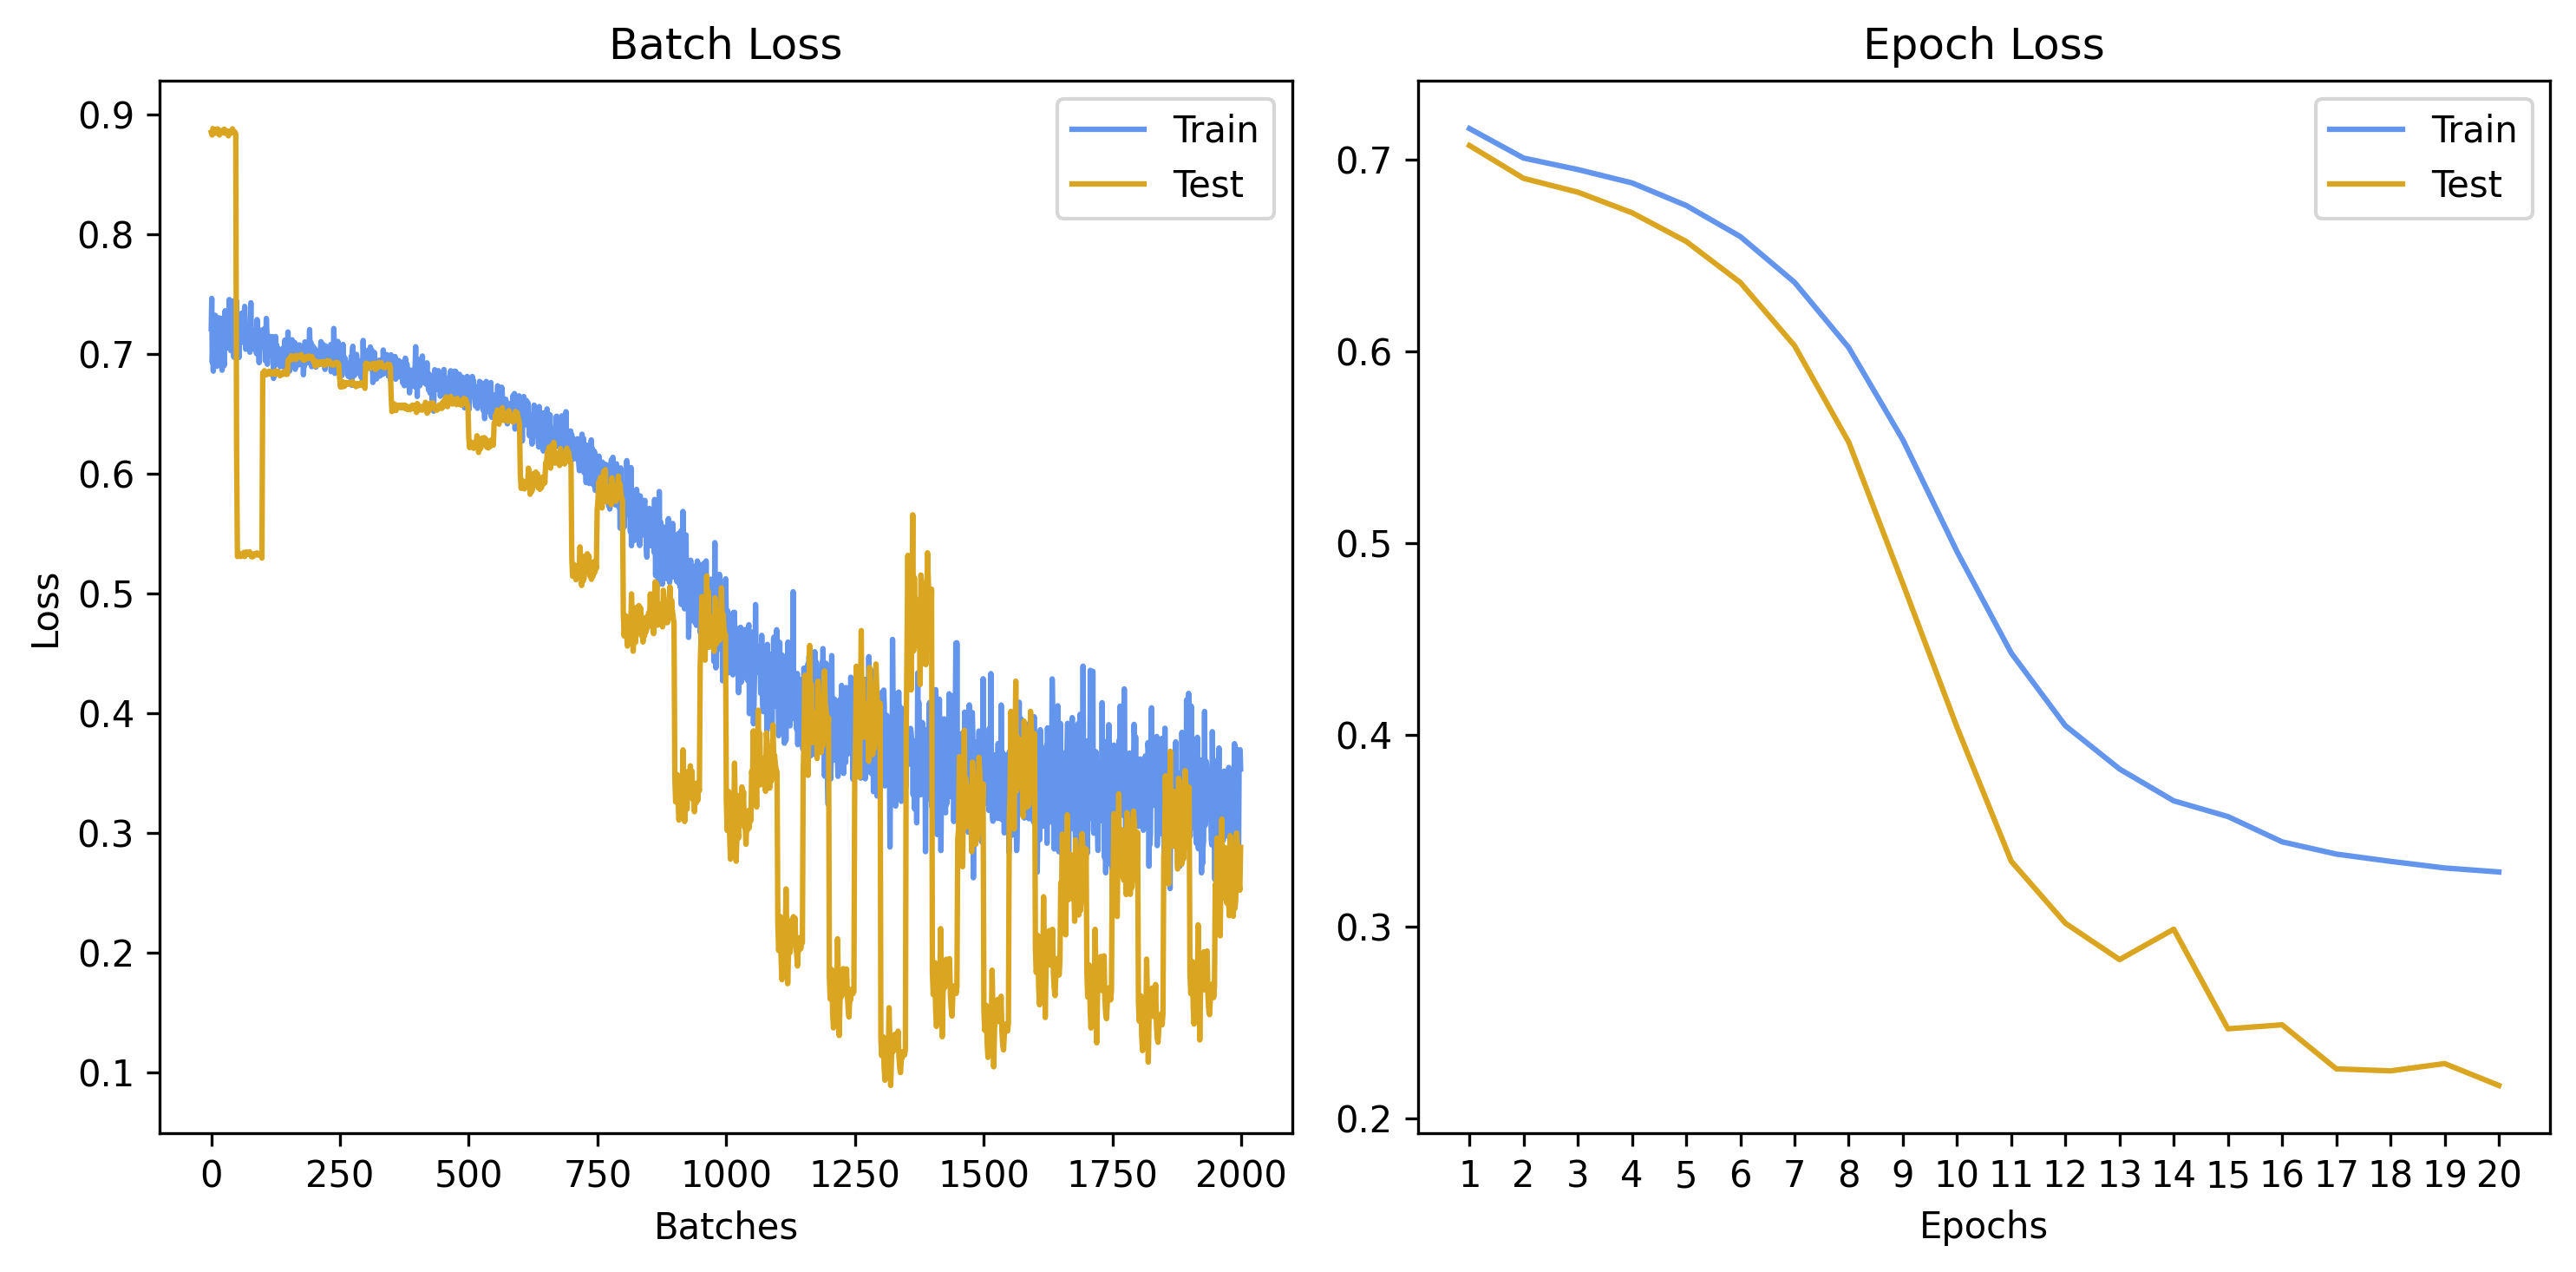
\includegraphics[width=\textwidth]{RoBERTa_learning_curves_1}
  \caption{Loss over training}
  \label{fig:roberta-learning-1}
\end{figure}

\begin{figure}
  \centering
  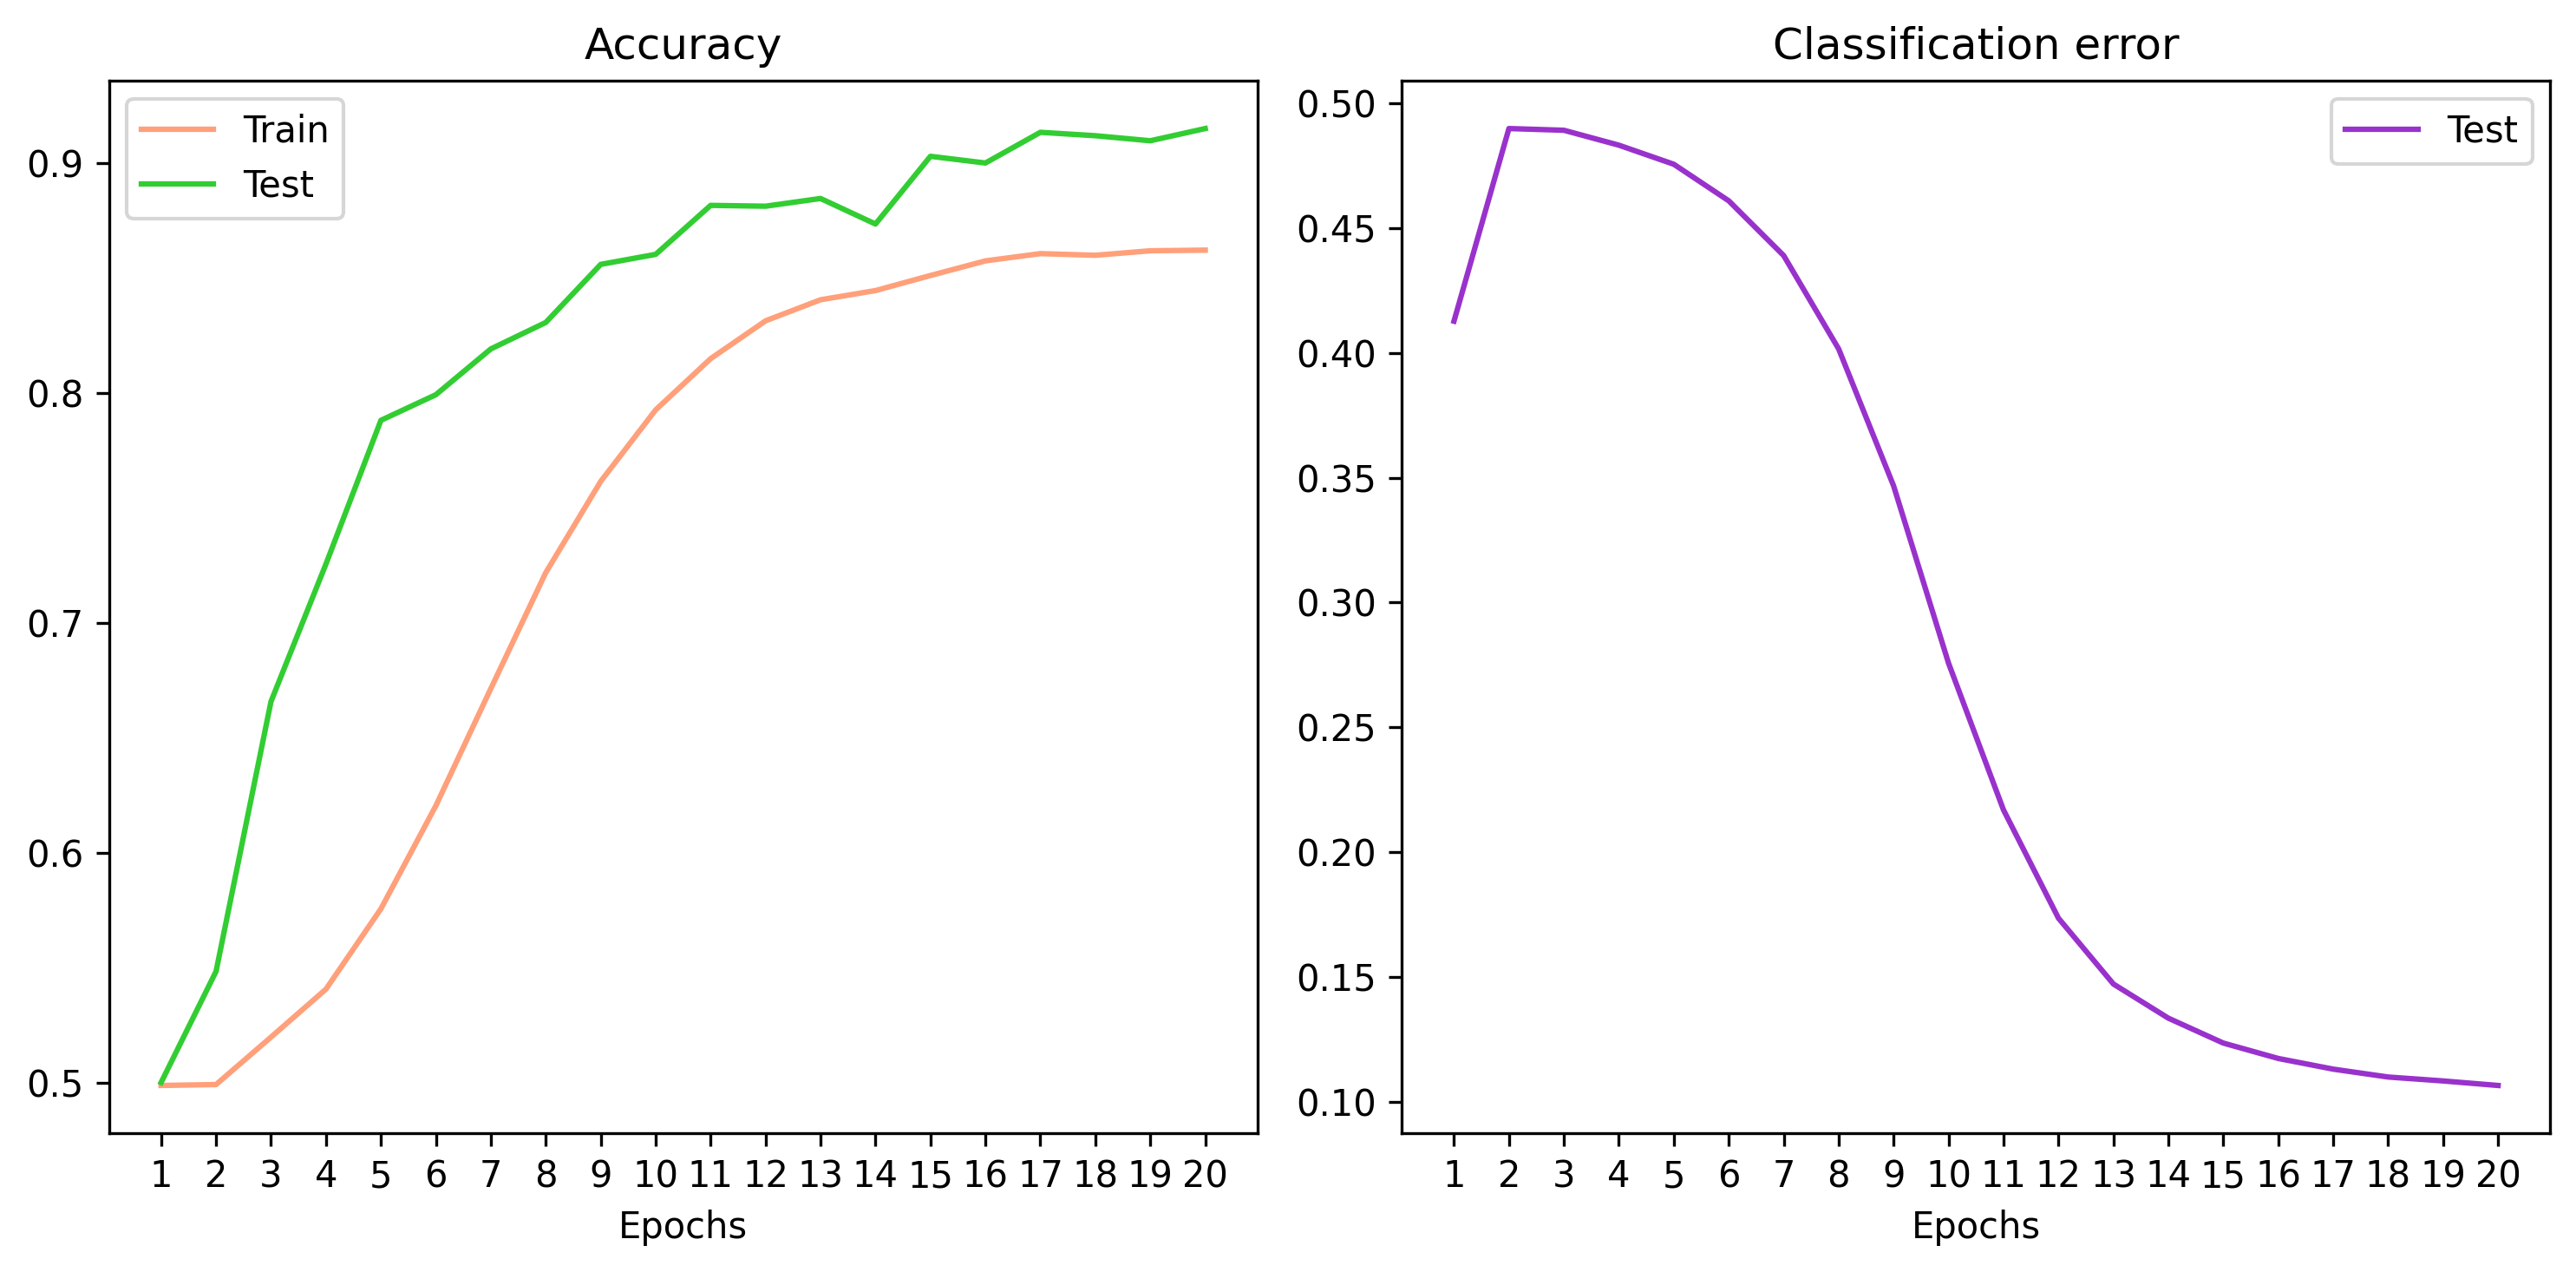
\includegraphics[width=\textwidth]{RoBERTa_learning_curves_2}
  \caption{Performance over training}
  \label{fig:roberta-learning-2}
\end{figure}

The behavior of the batch train loss can be attributed to the fact that test batches were not shuffled, unlike the training batches. It is quite obvious that some batches are more difficult to classify than others. However, since this only affects the test sample, it does not interfere with the training process. What is interesting, nonetheless, is that the difference between test batches continues to grow with each epoch, as if the model was improving for certain batches while plateauing on others.

Otherwise, 20 epochs seems to be quite a lot for fine-tuning, as typical values range between 3-5 epochs. This suggests that the model is converging slowly. However, the learning rate is relatively high, and warm-up steps were included, which makes that behavior somewhat perplexing (for reference, the values mentioned in the SOTA article for fine-tuning RoBERTa are 5 epochs with \texttt{lr=1e-6},  \texttt{batch\_size=16}, and \texttt{weight\_decay=0.01}) \citep{csanady_llambert_2024}. Investigating further was not possible due to the high computational cost.

The effect of training is notable on accuracy, but also on classification error, which reflects the separation between predicted classes, that is, the model confidence in its own predictions. Classification error is defined as the average difference between the highest possible probability (\( =1 \)) and the highest predicted probability of each datapoint (so the more certain are the label assignments, the closer \( E \) gets to 0):

\[
E = \frac{1}{N} \sum_{i=1}^{N} (1 - P_{\text{max},i})
\]

The overall improvement from fine-tuning is disappointing. While accuracy progresses significantly during training—from 0.5 after the first epoch (equivalent to random guessing, as the dataset is balanced) to 0.9152 after the 20\textsuperscript{th} epoch—it still falls short of the performance achieved by the base model with zero-shot classification, which is already at 0.9158. Moreover, it remains far below the performance of SiEBERT (0.9573) and the SOTA model (0.9668).

Several explanations can be conceived.
\begin{enumerate}
    \item The IMDb dataset is too small. Indeed, SiEBERT and the SOTA model are fine-tuned on bigger datasets. But it remains puzzling that even 20 epochs of fine-tuning does not yield better performance than the base model. 
	\item My classification head is inadequate. I tested an alternative model inspired by RoBERTa’s default classification head, consisting of 2 dense layers with a hidden size of 512. However, the performances of this model were notably worse after 12 epochs (0.8405 accuracy vs. 0.8841 for the original model, and 0.4195 vs. 0.2735 for classification error).
\end{enumerate}

I am unsure what else could have been done. I have reviewed many tutorials on fine-tuning BERT and RoBERTa, but none explicitly addressed its impact on accuracy---especially in comparison to zero-shot classification with optimized prompting. Perhaps fine-tuning RoBERTa effectively is harder than it seems.

\subsection{Performances}

I have introduced the performance of all models except GPT-3.5 Turbo. Its accuracy falls between zero-shot classification with optimized prompting and SiEBERT, highlighting that despite its capabilities and the use of advanced prompting techniques, specialized encoders can still outperform it. It would have been valuable to explore alternative prompt engineering strategies and test other GPT models. However, this was impractical due to the cost and the API's slow speed--—averaging 8 seconds per call, resulting in over 55 hours to process the entire dataset.

\begin{table}
  \caption{Overall performance of each model}
  \label{tab:overall_perfs}
  \centering
  \begin{tabular}{lc}
    \toprule
    Model & Accuracy \\
    \midrule
    RoBERTa fine-tuned & 0.9152 \\
    RoBERTa base & 0.9171 \\
    GPT 3.5 Turbo & 0.9300 \\
    SiEBERT & 0.9573 \\
    \bottomrule
  \end{tabular}
\end{table}

\subsubsection{By ratings}

A clear drop in performance is evident for ratings closer to neutral, as expected. However, the models exhibit notably different behaviors. The accuracy of RoBERTa-base, fine-tuned RoBERTa, and GPT-3.5 Turbo varies with the valence of reviews. RoBERTa-base and fine-tuned RoBERTa perform significantly better on positive reviews than on negative ones, whereas GPT-3.5 Turbo shows the opposite trend, excelling on negative reviews. These models also experience the largest performance declines on their weaker side: -31.9\% for RoBERTa-base, -25.1\% for fine-tuned RoBERTa, and -25.1\% for GPT-3.5 Turbo. SiEBERT, on the other hand, maintains similar performance for both negative and positive reviews, with comparable declines near neutral ratings. This consistency makes it not only the best-performing model but also the most stable across sentiment extremes.

\begin{table}
  \caption{Performance by sentiment}
  \label{tab:perfs_by_sentiment}
  \centering
  \begin{tabular}{lcc}
    \toprule
    \multirow{2}{*}{\centering Model} & \multicolumn{2}{c}{Sentiment} \\
    \cmidrule{2-3}
    & Negative & Positive \\
    \midrule
    RoBERTa fine-tuned & 0.892640 & 0.937760 \\
    RoBERTa base & 0.871040 & 0.963120 \\
    GPT & 0.962320 & 0.897760 \\
    SiEBERT & 0.952000 & 0.962640 \\
    \bottomrule
  \end{tabular}
\end{table}

This sheds a new light on the effects of fine-tuning. While it improved performance on negative reviews, it reduced it to a larger extent on positive ones. As a result, fine-tuning made the model more consistent, though not better overall. Regarding the GPT model, providing more positive examples than negative one in the prompt could have helped balance its performance.

\begin{figure}
  \centering
  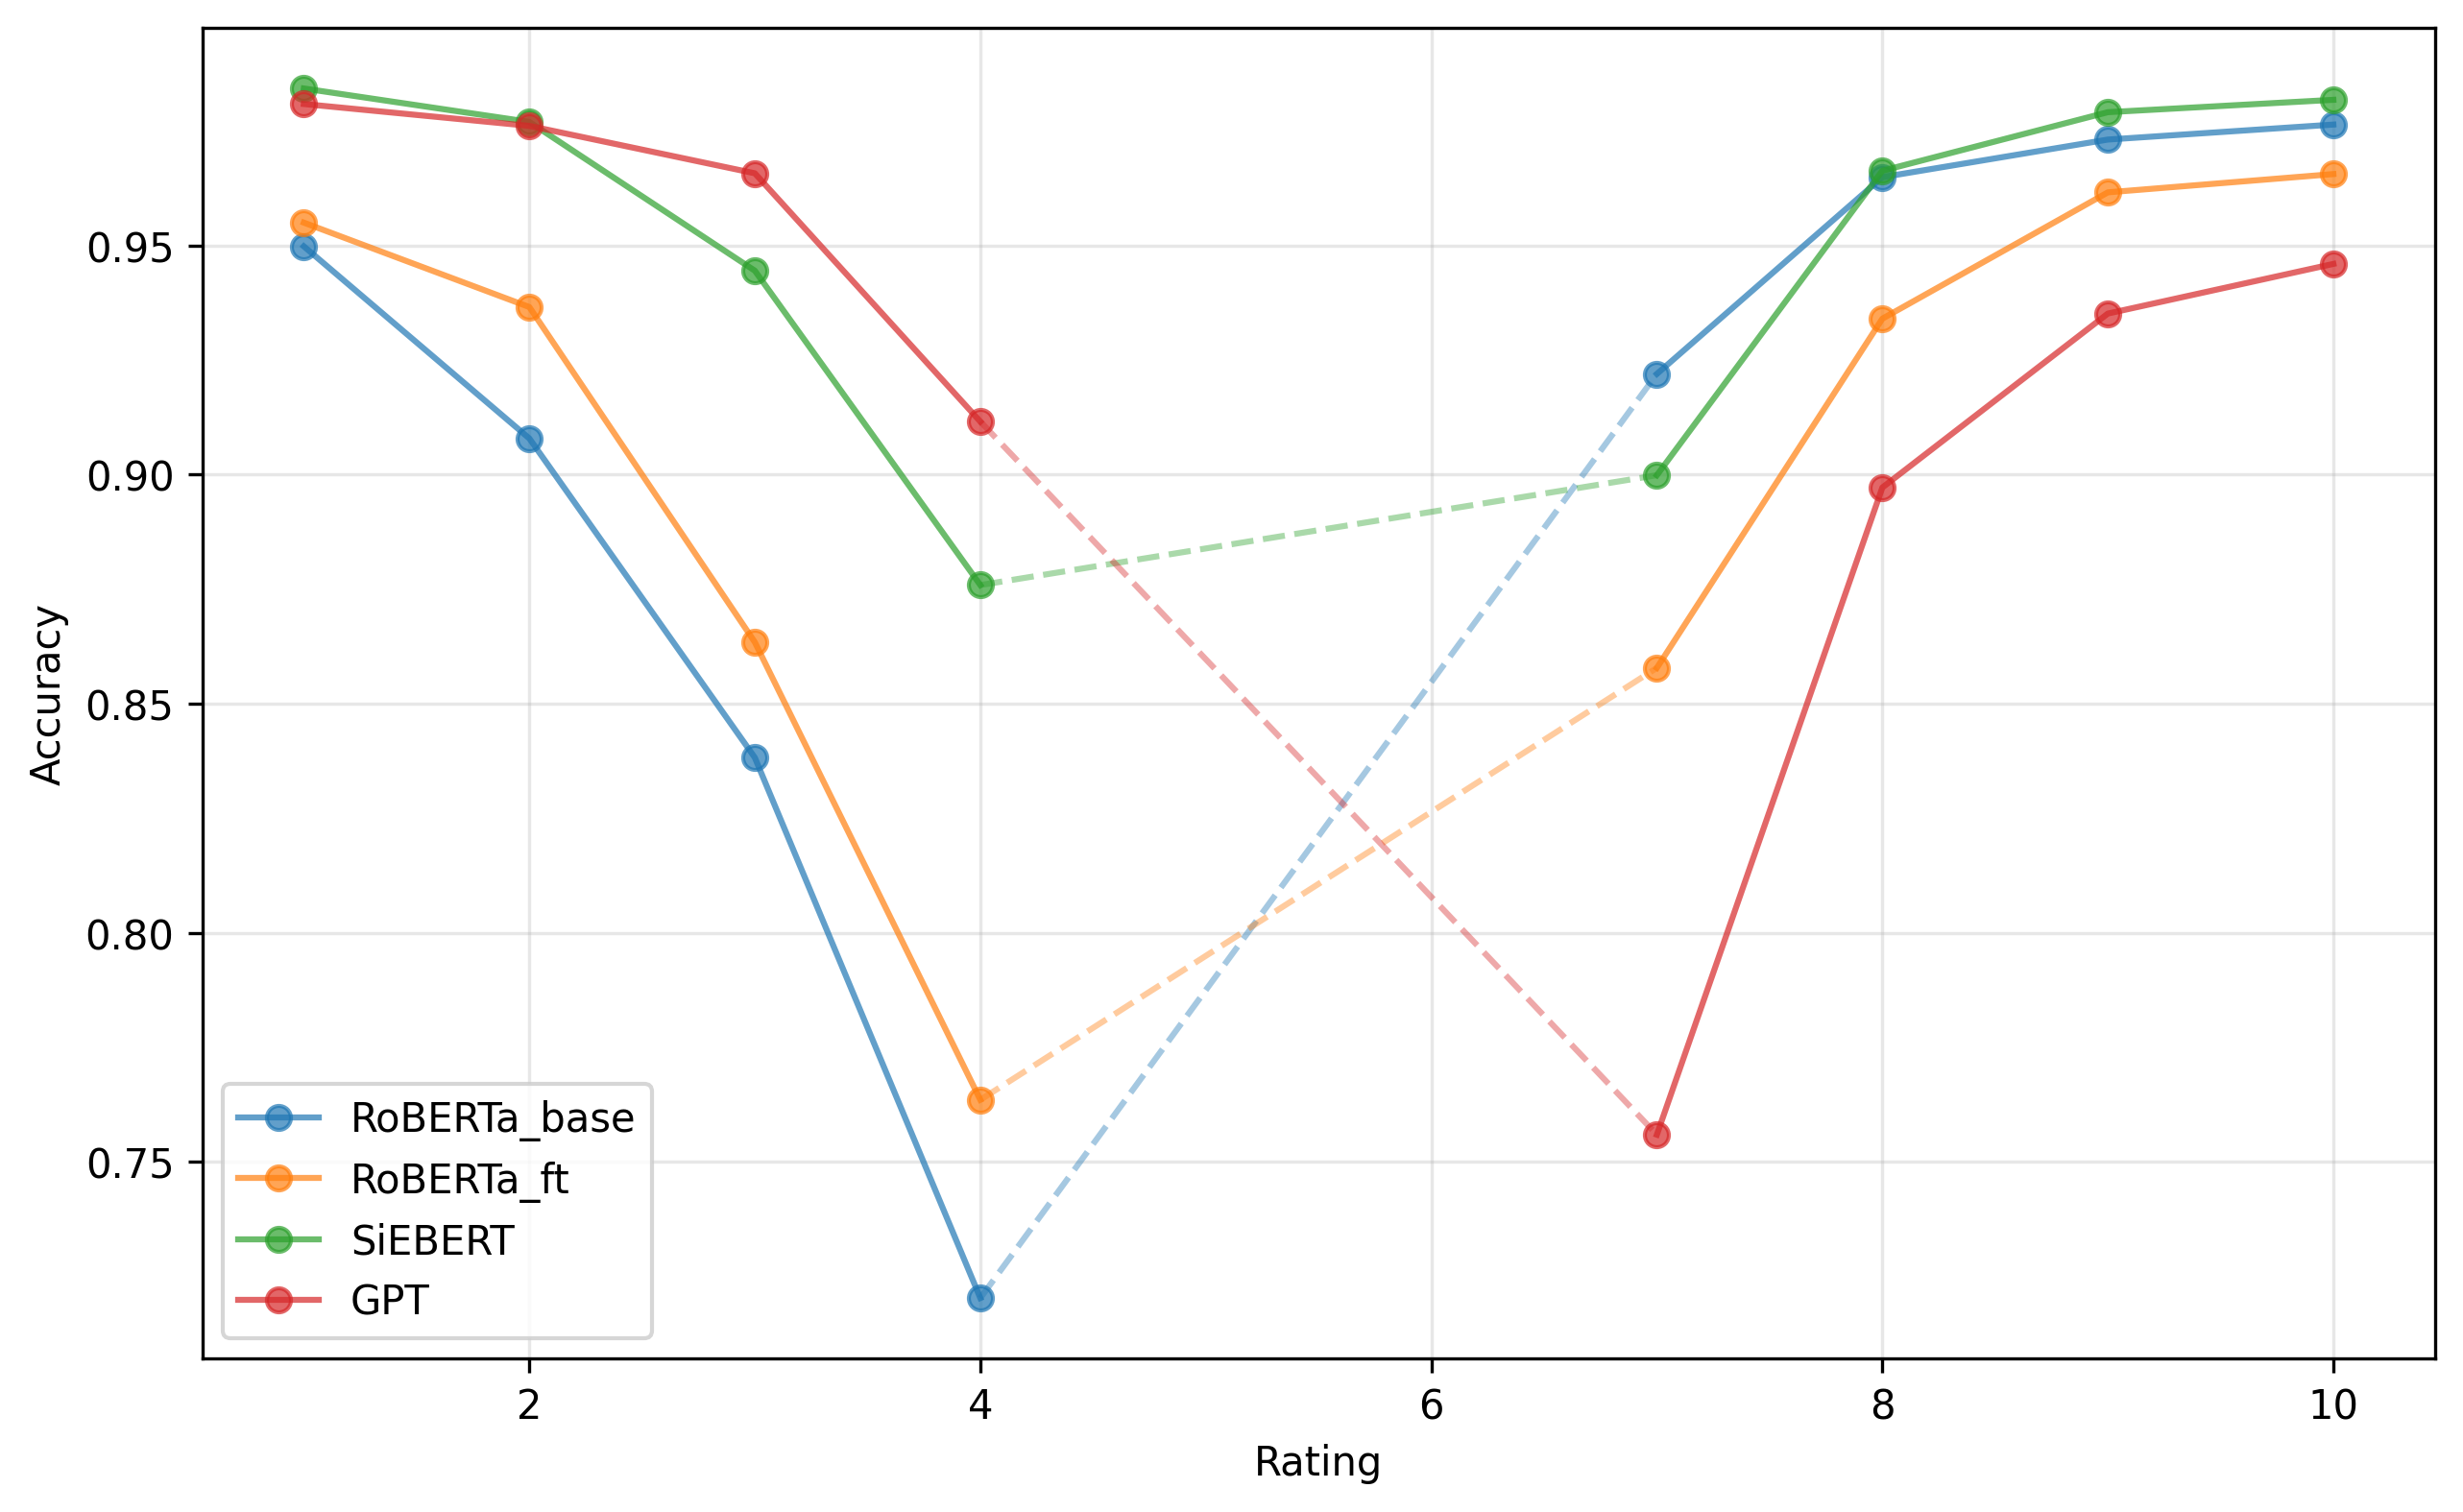
\includegraphics[width=\textwidth]{accuracy_vs_ratings.png}
  \caption{Accuracy by rating}
  \label{fig:roberta-accuracy-ratings}
\end{figure}

\subsubsection{By review length}

Similar observations emerge: SiEBERT maintains stable performance, while other models show a clear downward trend, though the effect of review length is much smaller than that of review valence. This aligns with the observation that truncation had minimal impact, suggesting that the key information in reviews is not heavily dependent on their length.

\begin{figure}
  \centering
  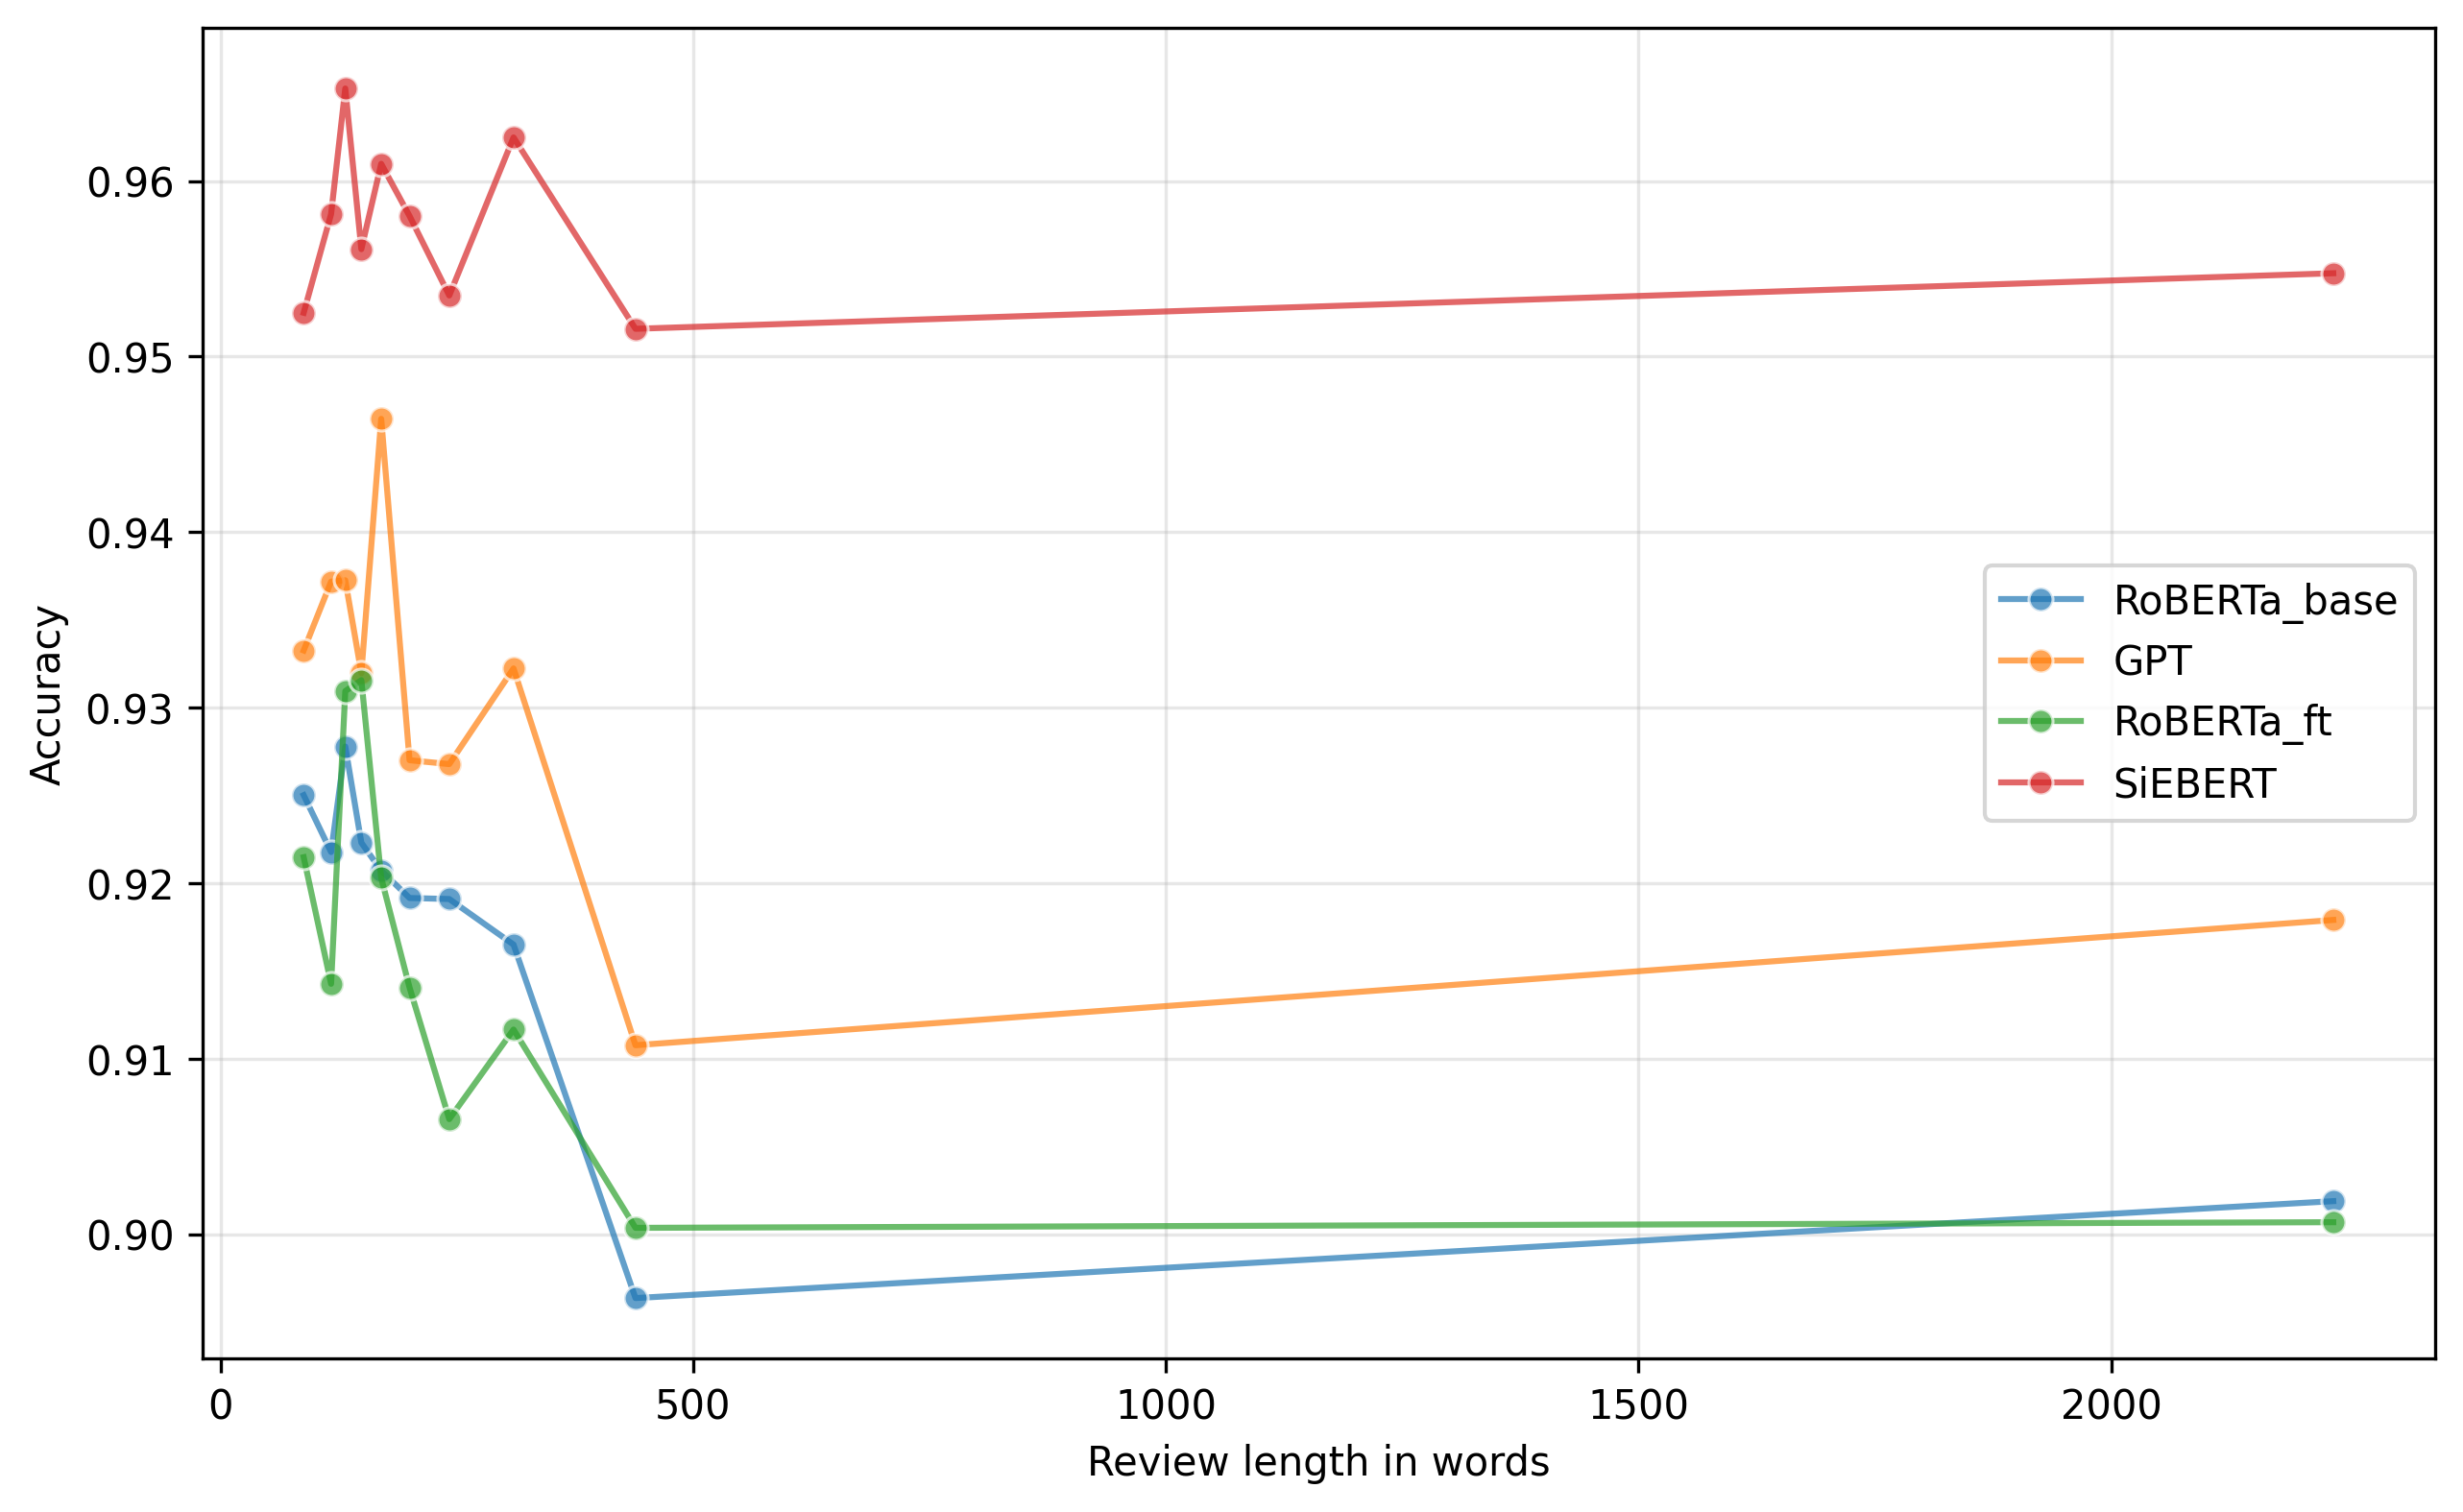
\includegraphics[width=\textwidth]{accuracy_vs_wordcount.png}
  \caption{Accuracy by review length}
  \label{fig:roberta-accuracy-length}
\end{figure}

\section{Discussion}

\bibliographystyle{unsrtnat}
\bibliography{references}

\end{document}



%%%%%%%%%%%%%%%%%%%%%%%%%%%%%%%%%%%%%%%%%%%%%%%%%



\section{Submission of papers to NeurIPS 2024}


Please read the instructions below carefully and follow them faithfully.


\subsection{Style}


Papers to be submitted to NeurIPS 2024 must be prepared according to the
instructions presented here. Papers may only be up to {\bf nine} pages long,
including figures. Additional pages \emph{containing only acknowledgments and
references} are allowed. Papers that exceed the page limit will not be
reviewed, or in any other way considered for presentation at the conference.


The margins in 2024 are the same as those in previous years.


Authors are required to use the NeurIPS \LaTeX{} style files obtainable at the
NeurIPS website as indicated below. Please make sure you use the current files
and not previous versions. Tweaking the style files may be grounds for
rejection.


\subsection{Retrieval of style files}


The style files for NeurIPS and other conference information are available on
the website at
\begin{center}
  \url{http://www.neurips.cc/}
\end{center}
The file \verb+neurips_2024.pdf+ contains these instructions and illustrates the
various formatting requirements your NeurIPS paper must satisfy.


The only supported style file for NeurIPS 2024 is \verb+neurips_2024.sty+,
rewritten for \LaTeXe{}.  \textbf{Previous style files for \LaTeX{} 2.09,
  Microsoft Word, and RTF are no longer supported!}


The \LaTeX{} style file contains three optional arguments: \verb+final+, which
creates a camera-ready copy, \verb+preprint+, which creates a preprint for
submission to, e.g., arXiv, and \verb+nonatbib+, which will not load the
\verb+natbib+ package for you in case of package clash.


\paragraph{Preprint option}
If you wish to post a preprint of your work online, e.g., on arXiv, using the
NeurIPS style, please use the \verb+preprint+ option. This will create a
nonanonymized version of your work with the text ``Preprint. Work in progress.''
in the footer. This version may be distributed as you see fit, as long as you do not say which conference it was submitted to. Please \textbf{do
  not} use the \verb+final+ option, which should \textbf{only} be used for
papers accepted to NeurIPS.


At submission time, please omit the \verb+final+ and \verb+preprint+
options. This will anonymize your submission and add line numbers to aid
review. Please do \emph{not} refer to these line numbers in your paper as they
will be removed during generation of camera-ready copies.


The file \verb+neurips_2024.tex+ may be used as a ``shell'' for writing your
paper. All you have to do is replace the author, title, abstract, and text of
the paper with your own.


The formatting instructions contained in these style files are summarized in
Sections \ref{gen_inst}, \ref{headings}, and \ref{others} below.


\section{General formatting instructions}
\label{gen_inst}


The text must be confined within a rectangle 5.5~inches (33~picas) wide and
9~inches (54~picas) long. The left margin is 1.5~inch (9~picas).  Use 10~point
type with a vertical spacing (leading) of 11~points.  Times New Roman is the
preferred typeface throughout, and will be selected for you by default.
Paragraphs are separated by \nicefrac{1}{2}~line space (5.5 points), with no
indentation.


The paper title should be 17~point, initial caps/lower case, bold, centered
between two horizontal rules. The top rule should be 4~points thick and the
bottom rule should be 1~point thick. Allow \nicefrac{1}{4}~inch space above and
below the title to rules. All pages should start at 1~inch (6~picas) from the
top of the page.


For the final version, authors' names are set in boldface, and each name is
centered above the corresponding address. The lead author's name is to be listed
first (left-most), and the co-authors' names (if different address) are set to
follow. If there is only one co-author, list both author and co-author side by
side.


Please pay special attention to the instructions in Section \ref{others}
regarding figures, tables, acknowledgments, and references.


\section{Headings: first level}
\label{headings}


All headings should be lower case (except for first word and proper nouns),
flush left, and bold.


First-level headings should be in 12-point type.


\subsection{Headings: second level}


Second-level headings should be in 10-point type.


\subsubsection{Headings: third level}


Third-level headings should be in 10-point type.


\paragraph{Paragraphs}


There is also a \verb+\paragraph+ command available, which sets the heading in
bold, flush left, and inline with the text, with the heading followed by 1\,em
of space.


\section{Citations, figures, tables, references}
\label{others}


These instructions apply to everyone.


\subsection{Citations within the text}


The \verb+natbib+ package will be loaded for you by default.  Citations may be
author/year or numeric, as long as you maintain internal consistency.  As to the
format of the references themselves, any style is acceptable as long as it is
used consistently.


The documentation for \verb+natbib+ may be found at
\begin{center}
  \url{http://mirrors.ctan.org/macros/latex/contrib/natbib/natnotes.pdf}
\end{center}
Of note is the command \verb+\citet+, which produces citations appropriate for
use in inline text.  For example,
\begin{verbatim}
   \citet{hasselmo} investigated\dots
\end{verbatim}
produces
\begin{quote}
  Hasselmo, et al.\ (1995) investigated\dots
\end{quote}


If you wish to load the \verb+natbib+ package with options, you may add the
following before loading the \verb+neurips_2024+ package:
\begin{verbatim}
   \PassOptionsToPackage{options}{natbib}
\end{verbatim}


If \verb+natbib+ clashes with another package you load, you can add the optional
argument \verb+nonatbib+ when loading the style file:
\begin{verbatim}
   \usepackage[nonatbib]{neurips_2024}
\end{verbatim}


As submission is double blind, refer to your own published work in the third
person. That is, use ``In the previous work of Jones et al.\ [4],'' not ``In our
previous work [4].'' If you cite your other papers that are not widely available
(e.g., a journal paper under review), use anonymous author names in the
citation, e.g., an author of the form ``A.\ Anonymous'' and include a copy of the anonymized paper in the supplementary material.


\subsection{Footnotes}


Footnotes should be used sparingly.  If you do require a footnote, indicate
footnotes with a number\footnote{Sample of the first footnote.} in the
text. Place the footnotes at the bottom of the page on which they appear.
Precede the footnote with a horizontal rule of 2~inches (12~picas).


Note that footnotes are properly typeset \emph{after} punctuation
marks.\footnote{As in this example.}


\subsection{Figures}


\begin{figure}
  \centering
  \fbox{\rule[-.5cm]{0cm}{4cm} \rule[-.5cm]{4cm}{0cm}}
  \caption{Sample figure caption.}
\end{figure}


All artwork must be neat, clean, and legible. Lines should be dark enough for
purposes of reproduction. The figure number and caption always appear after the
figure. Place one line space before the figure caption and one line space after
the figure. The figure caption should be lower case (except for first word and
proper nouns); figures are numbered consecutively.


You may use color figures.  However, it is best for the figure captions and the
paper body to be legible if the paper is printed in either black/white or in
color.


\subsection{Tables}


All tables must be centered, neat, clean and legible.  The table number and
title always appear before the table.  See Table~\ref{sample-table}.


Place one line space before the table title, one line space after the
table title, and one line space after the table. The table title must
be lower case (except for first word and proper nouns); tables are
numbered consecutively.


Note that publication-quality tables \emph{do not contain vertical rules.} We
strongly suggest the use of the \verb+booktabs+ package, which allows for
typesetting high-quality, professional tables:
\begin{center}
  \url{https://www.ctan.org/pkg/booktabs}
\end{center}
This package was used to typeset Table~\ref{sample-table}.


\begin{table}
  \caption{Sample table title}
  \label{sample-table}
  \centering
  \begin{tabular}{lll}
    \toprule
    \multicolumn{2}{c}{Part}                   \\
    \cmidrule(r){1-2}
    Name     & Description     & Size ($\mu$m) \\
    \midrule
    Dendrite & Input terminal  & $\sim$100     \\
    Axon     & Output terminal & $\sim$10      \\
    Soma     & Cell body       & up to $10^6$  \\
    \bottomrule
  \end{tabular}
\end{table}

\subsection{Math}
Note that display math in bare TeX commands will not create correct line numbers for submission. Please use LaTeX (or AMSTeX) commands for unnumbered display math. (You really shouldn't be using \$\$ anyway; see \url{https://tex.stackexchange.com/questions/503/why-is-preferable-to} and \url{https://tex.stackexchange.com/questions/40492/what-are-the-differences-between-align-equation-and-displaymath} for more information.)

\subsection{Final instructions}

Do not change any aspects of the formatting parameters in the style files.  In
particular, do not modify the width or length of the rectangle the text should
fit into, and do not change font sizes (except perhaps in the
\textbf{References} section; see below). Please note that pages should be
numbered.


\section{Preparing PDF files}


Please prepare submission files with paper size ``US Letter,'' and not, for
example, ``A4.''


Fonts were the main cause of problems in the past years. Your PDF file must only
contain Type 1 or Embedded TrueType fonts. Here are a few instructions to
achieve this.


\begin{itemize}


\item You should directly generate PDF files using \verb+pdflatex+.


\item You can check which fonts a PDF files uses.  In Acrobat Reader, select the
  menu Files$>$Document Properties$>$Fonts and select Show All Fonts. You can
  also use the program \verb+pdffonts+ which comes with \verb+xpdf+ and is
  available out-of-the-box on most Linux machines.


\item \verb+xfig+ "patterned" shapes are implemented with bitmap fonts.  Use
  "solid" shapes instead.


\item The \verb+\bbold+ package almost always uses bitmap fonts.  You should use
  the equivalent AMS Fonts:
\begin{verbatim}
   \usepackage{amsfonts}
\end{verbatim}
followed by, e.g., \verb+\mathbb{R}+, \verb+\mathbb{N}+, or \verb+\mathbb{C}+
for $\mathbb{R}$, $\mathbb{N}$ or $\mathbb{C}$.  You can also use the following
workaround for reals, natural and complex:
\begin{verbatim}
   \newcommand{\RR}{I\!\!R} %real numbers
   \newcommand{\Nat}{I\!\!N} %natural numbers
   \newcommand{\CC}{I\!\!\!\!C} %complex numbers
\end{verbatim}
Note that \verb+amsfonts+ is automatically loaded by the \verb+amssymb+ package.


\end{itemize}


If your file contains type 3 fonts or non embedded TrueType fonts, we will ask
you to fix it.


\subsection{Margins in \LaTeX{}}


Most of the margin problems come from figures positioned by hand using
\verb+\special+ or other commands. We suggest using the command
\verb+\includegraphics+ from the \verb+graphicx+ package. Always specify the
figure width as a multiple of the line width as in the example below:
\begin{verbatim}
   \usepackage[pdftex]{graphicx} ...
   \includegraphics[width=0.8\linewidth]{myfile.pdf}
\end{verbatim}
See Section 4.4 in the graphics bundle documentation
(\url{http://mirrors.ctan.org/macros/latex/required/graphics/grfguide.pdf})


A number of width problems arise when \LaTeX{} cannot properly hyphenate a
line. Please give LaTeX hyphenation hints using the \verb+\-+ command when
necessary.

\begin{ack}
Use unnumbered first level headings for the acknowledgments. All acknowledgments
go at the end of the paper before the list of references. Moreover, you are required to declare
funding (financial activities supporting the submitted work) and competing interests (related financial activities outside the submitted work).
More information about this disclosure can be found at: \url{https://neurips.cc/Conferences/2024/PaperInformation/FundingDisclosure}.


Do {\bf not} include this section in the anonymized submission, only in the final paper. You can use the \texttt{ack} environment provided in the style file to automatically hide this section in the anonymized submission.
\end{ack}

\section*{References}


References follow the acknowledgments in the camera-ready paper. Use unnumbered first-level heading for
the references. Any choice of citation style is acceptable as long as you are
consistent. It is permissible to reduce the font size to \verb+small+ (9 point)
when listing the references.
Note that the Reference section does not count towards the page limit.
\medskip


{
\small


[1] Alexander, J.A.\ \& Mozer, M.C.\ (1995) Template-based algorithms for
connectionist rule extraction. In G.\ Tesauro, D.S.\ Touretzky and T.K.\ Leen
(eds.), {\it Advances in Neural Information Processing Systems 7},
pp.\ 609--616. Cambridge, MA: MIT Press.


[2] Bower, J.M.\ \& Beeman, D.\ (1995) {\it The Book of GENESIS: Exploring
  Realistic Neural Models with the GEneral NEural SImulation System.}  New York:
TELOS/Springer--Verlag.


[3] Hasselmo, M.E., Schnell, E.\ \& Barkai, E.\ (1995) Dynamics of learning and
recall at excitatory recurrent synapses and cholinergic modulation in rat
hippocampal region CA3. {\it Journal of Neuroscience} {\bf 15}(7):5249-5262.
}


%%%%%%%%%%%%%%%%%%%%%%%%%%%%%%%%%%%%%%%%%%%%%%%%%%%%%%%%%%%%

\appendix

\section{Appendix / supplemental material}


Optionally include supplemental material (complete proofs, additional experiments and plots) in appendix.
All such materials \textbf{SHOULD be included in the main submission.}

%%%%%%%%%%%%%%%%%%%%%%%%%%%%%%%%%%%%%%%%%%%%%%%%%%%%%%%%%%%%

\newpage
\section*{NeurIPS Paper Checklist}

%%% BEGIN INSTRUCTIONS %%%
The checklist is designed to encourage best practices for responsible machine learning research, addressing issues of reproducibility, transparency, research ethics, and societal impact. Do not remove the checklist: {\bf The papers not including the checklist will be desk rejected.} The checklist should follow the references and follow the (optional) supplemental material.  The checklist does NOT count towards the page
limit. 

Please read the checklist guidelines carefully for information on how to answer these questions. For each question in the checklist:
\begin{itemize}
    \item You should answer \answerYes{}, \answerNo{}, or \answerNA{}.
    \item \answerNA{} means either that the question is Not Applicable for that particular paper or the relevant information is Not Available.
    \item Please provide a short (1–2 sentence) justification right after your answer (even for NA). 
   % \item {\bf The papers not including the checklist will be desk rejected.}
\end{itemize}

{\bf The checklist answers are an integral part of your paper submission.} They are visible to the reviewers, area chairs, senior area chairs, and ethics reviewers. You will be asked to also include it (after eventual revisions) with the final version of your paper, and its final version will be published with the paper.

The reviewers of your paper will be asked to use the checklist as one of the factors in their evaluation. While "\answerYes{}" is generally preferable to "\answerNo{}", it is perfectly acceptable to answer "\answerNo{}" provided a proper justification is given (e.g., "error bars are not reported because it would be too computationally expensive" or "we were unable to find the license for the dataset we used"). In general, answering "\answerNo{}" or "\answerNA{}" is not grounds for rejection. While the questions are phrased in a binary way, we acknowledge that the true answer is often more nuanced, so please just use your best judgment and write a justification to elaborate. All supporting evidence can appear either in the main paper or the supplemental material, provided in appendix. If you answer \answerYes{} to a question, in the justification please point to the section(s) where related material for the question can be found.

IMPORTANT, please:
\begin{itemize}
    \item {\bf Delete this instruction block, but keep the section heading ``NeurIPS paper checklist"},
    \item  {\bf Keep the checklist subsection headings, questions/answers and guidelines below.}
    \item {\bf Do not modify the questions and only use the provided macros for your answers}.
\end{itemize} 
 

%%% END INSTRUCTIONS %%%


\begin{enumerate}

\item {\bf Claims}
    \item[] Question: Do the main claims made in the abstract and introduction accurately reflect the paper's contributions and scope?
    \item[] Answer: \answerTODO{} % Replace by \answerYes{}, \answerNo{}, or \answerNA{}.
    \item[] Justification: \justificationTODO{}
    \item[] Guidelines:
    \begin{itemize}
        \item The answer NA means that the abstract and introduction do not include the claims made in the paper.
        \item The abstract and/or introduction should clearly state the claims made, including the contributions made in the paper and important assumptions and limitations. A No or NA answer to this question will not be perceived well by the reviewers. 
        \item The claims made should match theoretical and experimental results, and reflect how much the results can be expected to generalize to other settings. 
        \item It is fine to include aspirational goals as motivation as long as it is clear that these goals are not attained by the paper. 
    \end{itemize}

\item {\bf Limitations}
    \item[] Question: Does the paper discuss the limitations of the work performed by the authors?
    \item[] Answer: \answerTODO{} % Replace by \answerYes{}, \answerNo{}, or \answerNA{}.
    \item[] Justification: \justificationTODO{}
    \item[] Guidelines:
    \begin{itemize}
        \item The answer NA means that the paper has no limitation while the answer No means that the paper has limitations, but those are not discussed in the paper. 
        \item The authors are encouraged to create a separate "Limitations" section in their paper.
        \item The paper should point out any strong assumptions and how robust the results are to violations of these assumptions (e.g., independence assumptions, noiseless settings, model well-specification, asymptotic approximations only holding locally). The authors should reflect on how these assumptions might be violated in practice and what the implications would be.
        \item The authors should reflect on the scope of the claims made, e.g., if the approach was only tested on a few datasets or with a few runs. In general, empirical results often depend on implicit assumptions, which should be articulated.
        \item The authors should reflect on the factors that influence the performance of the approach. For example, a facial recognition algorithm may perform poorly when image resolution is low or images are taken in low lighting. Or a speech-to-text system might not be used reliably to provide closed captions for online lectures because it fails to handle technical jargon.
        \item The authors should discuss the computational efficiency of the proposed algorithms and how they scale with dataset size.
        \item If applicable, the authors should discuss possible limitations of their approach to address problems of privacy and fairness.
        \item While the authors might fear that complete honesty about limitations might be used by reviewers as grounds for rejection, a worse outcome might be that reviewers discover limitations that aren't acknowledged in the paper. The authors should use their best judgment and recognize that individual actions in favor of transparency play an important role in developing norms that preserve the integrity of the community. Reviewers will be specifically instructed to not penalize honesty concerning limitations.
    \end{itemize}

\item {\bf Theory Assumptions and Proofs}
    \item[] Question: For each theoretical result, does the paper provide the full set of assumptions and a complete (and correct) proof?
    \item[] Answer: \answerTODO{} % Replace by \answerYes{}, \answerNo{}, or \answerNA{}.
    \item[] Justification: \justificationTODO{}
    \item[] Guidelines:
    \begin{itemize}
        \item The answer NA means that the paper does not include theoretical results. 
        \item All the theorems, formulas, and proofs in the paper should be numbered and cross-referenced.
        \item All assumptions should be clearly stated or referenced in the statement of any theorems.
        \item The proofs can either appear in the main paper or the supplemental material, but if they appear in the supplemental material, the authors are encouraged to provide a short proof sketch to provide intuition. 
        \item Inversely, any informal proof provided in the core of the paper should be complemented by formal proofs provided in appendix or supplemental material.
        \item Theorems and Lemmas that the proof relies upon should be properly referenced. 
    \end{itemize}

    \item {\bf Experimental Result Reproducibility}
    \item[] Question: Does the paper fully disclose all the information needed to reproduce the main experimental results of the paper to the extent that it affects the main claims and/or conclusions of the paper (regardless of whether the code and data are provided or not)?
    \item[] Answer: \answerTODO{} % Replace by \answerYes{}, \answerNo{}, or \answerNA{}.
    \item[] Justification: \justificationTODO{}
    \item[] Guidelines:
    \begin{itemize}
        \item The answer NA means that the paper does not include experiments.
        \item If the paper includes experiments, a No answer to this question will not be perceived well by the reviewers: Making the paper reproducible is important, regardless of whether the code and data are provided or not.
        \item If the contribution is a dataset and/or model, the authors should describe the steps taken to make their results reproducible or verifiable. 
        \item Depending on the contribution, reproducibility can be accomplished in various ways. For example, if the contribution is a novel architecture, describing the architecture fully might suffice, or if the contribution is a specific model and empirical evaluation, it may be necessary to either make it possible for others to replicate the model with the same dataset, or provide access to the model. In general. releasing code and data is often one good way to accomplish this, but reproducibility can also be provided via detailed instructions for how to replicate the results, access to a hosted model (e.g., in the case of a large language model), releasing of a model checkpoint, or other means that are appropriate to the research performed.
        \item While NeurIPS does not require releasing code, the conference does require all submissions to provide some reasonable avenue for reproducibility, which may depend on the nature of the contribution. For example
        \begin{enumerate}
            \item If the contribution is primarily a new algorithm, the paper should make it clear how to reproduce that algorithm.
            \item If the contribution is primarily a new model architecture, the paper should describe the architecture clearly and fully.
            \item If the contribution is a new model (e.g., a large language model), then there should either be a way to access this model for reproducing the results or a way to reproduce the model (e.g., with an open-source dataset or instructions for how to construct the dataset).
            \item We recognize that reproducibility may be tricky in some cases, in which case authors are welcome to describe the particular way they provide for reproducibility. In the case of closed-source models, it may be that access to the model is limited in some way (e.g., to registered users), but it should be possible for other researchers to have some path to reproducing or verifying the results.
        \end{enumerate}
    \end{itemize}


\item {\bf Open access to data and code}
    \item[] Question: Does the paper provide open access to the data and code, with sufficient instructions to faithfully reproduce the main experimental results, as described in supplemental material?
    \item[] Answer: \answerTODO{} % Replace by \answerYes{}, \answerNo{}, or \answerNA{}.
    \item[] Justification: \justificationTODO{}
    \item[] Guidelines:
    \begin{itemize}
        \item The answer NA means that paper does not include experiments requiring code.
        \item Please see the NeurIPS code and data submission guidelines (\url{https://nips.cc/public/guides/CodeSubmissionPolicy}) for more details.
        \item While we encourage the release of code and data, we understand that this might not be possible, so “No” is an acceptable answer. Papers cannot be rejected simply for not including code, unless this is central to the contribution (e.g., for a new open-source benchmark).
        \item The instructions should contain the exact command and environment needed to run to reproduce the results. See the NeurIPS code and data submission guidelines (\url{https://nips.cc/public/guides/CodeSubmissionPolicy}) for more details.
        \item The authors should provide instructions on data access and preparation, including how to access the raw data, preprocessed data, intermediate data, and generated data, etc.
        \item The authors should provide scripts to reproduce all experimental results for the new proposed method and baselines. If only a subset of experiments are reproducible, they should state which ones are omitted from the script and why.
        \item At submission time, to preserve anonymity, the authors should release anonymized versions (if applicable).
        \item Providing as much information as possible in supplemental material (appended to the paper) is recommended, but including URLs to data and code is permitted.
    \end{itemize}


\item {\bf Experimental Setting/Details}
    \item[] Question: Does the paper specify all the training and test details (e.g., data splits, hyperparameters, how they were chosen, type of optimizer, etc.) necessary to understand the results?
    \item[] Answer: \answerTODO{} % Replace by \answerYes{}, \answerNo{}, or \answerNA{}.
    \item[] Justification: \justificationTODO{}
    \item[] Guidelines:
    \begin{itemize}
        \item The answer NA means that the paper does not include experiments.
        \item The experimental setting should be presented in the core of the paper to a level of detail that is necessary to appreciate the results and make sense of them.
        \item The full details can be provided either with the code, in appendix, or as supplemental material.
    \end{itemize}

\item {\bf Experiment Statistical Significance}
    \item[] Question: Does the paper report error bars suitably and correctly defined or other appropriate information about the statistical significance of the experiments?
    \item[] Answer: \answerTODO{} % Replace by \answerYes{}, \answerNo{}, or \answerNA{}.
    \item[] Justification: \justificationTODO{}
    \item[] Guidelines:
    \begin{itemize}
        \item The answer NA means that the paper does not include experiments.
        \item The authors should answer "Yes" if the results are accompanied by error bars, confidence intervals, or statistical significance tests, at least for the experiments that support the main claims of the paper.
        \item The factors of variability that the error bars are capturing should be clearly stated (for example, train/test split, initialization, random drawing of some parameter, or overall run with given experimental conditions).
        \item The method for calculating the error bars should be explained (closed form formula, call to a library function, bootstrap, etc.)
        \item The assumptions made should be given (e.g., Normally distributed errors).
        \item It should be clear whether the error bar is the standard deviation or the standard error of the mean.
        \item It is OK to report 1-sigma error bars, but one should state it. The authors should preferably report a 2-sigma error bar than state that they have a 96\% CI, if the hypothesis of Normality of errors is not verified.
        \item For asymmetric distributions, the authors should be careful not to show in tables or figures symmetric error bars that would yield results that are out of range (e.g. negative error rates).
        \item If error bars are reported in tables or plots, The authors should explain in the text how they were calculated and reference the corresponding figures or tables in the text.
    \end{itemize}

\item {\bf Experiments Compute Resources}
    \item[] Question: For each experiment, does the paper provide sufficient information on the computer resources (type of compute workers, memory, time of execution) needed to reproduce the experiments?
    \item[] Answer: \answerTODO{} % Replace by \answerYes{}, \answerNo{}, or \answerNA{}.
    \item[] Justification: \justificationTODO{}
    \item[] Guidelines:
    \begin{itemize}
        \item The answer NA means that the paper does not include experiments.
        \item The paper should indicate the type of compute workers CPU or GPU, internal cluster, or cloud provider, including relevant memory and storage.
        \item The paper should provide the amount of compute required for each of the individual experimental runs as well as estimate the total compute. 
        \item The paper should disclose whether the full research project required more compute than the experiments reported in the paper (e.g., preliminary or failed experiments that didn't make it into the paper). 
    \end{itemize}
    
\item {\bf Code Of Ethics}
    \item[] Question: Does the research conducted in the paper conform, in every respect, with the NeurIPS Code of Ethics \url{https://neurips.cc/public/EthicsGuidelines}?
    \item[] Answer: \answerTODO{} % Replace by \answerYes{}, \answerNo{}, or \answerNA{}.
    \item[] Justification: \justificationTODO{}
    \item[] Guidelines:
    \begin{itemize}
        \item The answer NA means that the authors have not reviewed the NeurIPS Code of Ethics.
        \item If the authors answer No, they should explain the special circumstances that require a deviation from the Code of Ethics.
        \item The authors should make sure to preserve anonymity (e.g., if there is a special consideration due to laws or regulations in their jurisdiction).
    \end{itemize}


\item {\bf Broader Impacts}
    \item[] Question: Does the paper discuss both potential positive societal impacts and negative societal impacts of the work performed?
    \item[] Answer: \answerTODO{} % Replace by \answerYes{}, \answerNo{}, or \answerNA{}.
    \item[] Justification: \justificationTODO{}
    \item[] Guidelines:
    \begin{itemize}
        \item The answer NA means that there is no societal impact of the work performed.
        \item If the authors answer NA or No, they should explain why their work has no societal impact or why the paper does not address societal impact.
        \item Examples of negative societal impacts include potential malicious or unintended uses (e.g., disinformation, generating fake profiles, surveillance), fairness considerations (e.g., deployment of technologies that could make decisions that unfairly impact specific groups), privacy considerations, and security considerations.
        \item The conference expects that many papers will be foundational research and not tied to particular applications, let alone deployments. However, if there is a direct path to any negative applications, the authors should point it out. For example, it is legitimate to point out that an improvement in the quality of generative models could be used to generate deepfakes for disinformation. On the other hand, it is not needed to point out that a generic algorithm for optimizing neural networks could enable people to train models that generate Deepfakes faster.
        \item The authors should consider possible harms that could arise when the technology is being used as intended and functioning correctly, harms that could arise when the technology is being used as intended but gives incorrect results, and harms following from (intentional or unintentional) misuse of the technology.
        \item If there are negative societal impacts, the authors could also discuss possible mitigation strategies (e.g., gated release of models, providing defenses in addition to attacks, mechanisms for monitoring misuse, mechanisms to monitor how a system learns from feedback over time, improving the efficiency and accessibility of ML).
    \end{itemize}
    
\item {\bf Safeguards}
    \item[] Question: Does the paper describe safeguards that have been put in place for responsible release of data or models that have a high risk for misuse (e.g., pretrained language models, image generators, or scraped datasets)?
    \item[] Answer: \answerTODO{} % Replace by \answerYes{}, \answerNo{}, or \answerNA{}.
    \item[] Justification: \justificationTODO{}
    \item[] Guidelines:
    \begin{itemize}
        \item The answer NA means that the paper poses no such risks.
        \item Released models that have a high risk for misuse or dual-use should be released with necessary safeguards to allow for controlled use of the model, for example by requiring that users adhere to usage guidelines or restrictions to access the model or implementing safety filters. 
        \item Datasets that have been scraped from the Internet could pose safety risks. The authors should describe how they avoided releasing unsafe images.
        \item We recognize that providing effective safeguards is challenging, and many papers do not require this, but we encourage authors to take this into account and make a best faith effort.
    \end{itemize}

\item {\bf Licenses for existing assets}
    \item[] Question: Are the creators or original owners of assets (e.g., code, data, models), used in the paper, properly credited and are the license and terms of use explicitly mentioned and properly respected?
    \item[] Answer: \answerTODO{} % Replace by \answerYes{}, \answerNo{}, or \answerNA{}.
    \item[] Justification: \justificationTODO{}
    \item[] Guidelines:
    \begin{itemize}
        \item The answer NA means that the paper does not use existing assets.
        \item The authors should cite the original paper that produced the code package or dataset.
        \item The authors should state which version of the asset is used and, if possible, include a URL.
        \item The name of the license (e.g., CC-BY 4.0) should be included for each asset.
        \item For scraped data from a particular source (e.g., website), the copyright and terms of service of that source should be provided.
        \item If assets are released, the license, copyright information, and terms of use in the package should be provided. For popular datasets, \url{paperswithcode.com/datasets} has curated licenses for some datasets. Their licensing guide can help determine the license of a dataset.
        \item For existing datasets that are re-packaged, both the original license and the license of the derived asset (if it has changed) should be provided.
        \item If this information is not available online, the authors are encouraged to reach out to the asset's creators.
    \end{itemize}

\item {\bf New Assets}
    \item[] Question: Are new assets introduced in the paper well documented and is the documentation provided alongside the assets?
    \item[] Answer: \answerTODO{} % Replace by \answerYes{}, \answerNo{}, or \answerNA{}.
    \item[] Justification: \justificationTODO{}
    \item[] Guidelines:
    \begin{itemize}
        \item The answer NA means that the paper does not release new assets.
        \item Researchers should communicate the details of the dataset/code/model as part of their submissions via structured templates. This includes details about training, license, limitations, etc. 
        \item The paper should discuss whether and how consent was obtained from people whose asset is used.
        \item At submission time, remember to anonymize your assets (if applicable). You can either create an anonymized URL or include an anonymized zip file.
    \end{itemize}

\item {\bf Crowdsourcing and Research with Human Subjects}
    \item[] Question: For crowdsourcing experiments and research with human subjects, does the paper include the full text of instructions given to participants and screenshots, if applicable, as well as details about compensation (if any)? 
    \item[] Answer: \answerTODO{} % Replace by \answerYes{}, \answerNo{}, or \answerNA{}.
    \item[] Justification: \justificationTODO{}
    \item[] Guidelines:
    \begin{itemize}
        \item The answer NA means that the paper does not involve crowdsourcing nor research with human subjects.
        \item Including this information in the supplemental material is fine, but if the main contribution of the paper involves human subjects, then as much detail as possible should be included in the main paper. 
        \item According to the NeurIPS Code of Ethics, workers involved in data collection, curation, or other labor should be paid at least the minimum wage in the country of the data collector. 
    \end{itemize}

\item {\bf Institutional Review Board (IRB) Approvals or Equivalent for Research with Human Subjects}
    \item[] Question: Does the paper describe potential risks incurred by study participants, whether such risks were disclosed to the subjects, and whether Institutional Review Board (IRB) approvals (or an equivalent approval/review based on the requirements of your country or institution) were obtained?
    \item[] Answer: \answerTODO{} % Replace by \answerYes{}, \answerNo{}, or \answerNA{}.
    \item[] Justification: \justificationTODO{}
    \item[] Guidelines:
    \begin{itemize}
        \item The answer NA means that the paper does not involve crowdsourcing nor research with human subjects.
        \item Depending on the country in which research is conducted, IRB approval (or equivalent) may be required for any human subjects research. If you obtained IRB approval, you should clearly state this in the paper. 
        \item We recognize that the procedures for this may vary significantly between institutions and locations, and we expect authors to adhere to the NeurIPS Code of Ethics and the guidelines for their institution. 
        \item For initial submissions, do not include any information that would break anonymity (if applicable), such as the institution conducting the review.
    \end{itemize}

\end{enumerate}


\end{document}
